 \section{Propuesta}
\subsection{Requerimientos}
\begin{frame}{Propuesta de solución}
	\begin{block}{El desarrollador requiere}
		\begin{itemize}
		  \item Definir políticas de seguridad desde la implementación de sus aplicativos.
		  \item Una herramienta que verifique las políticas definidas.
		  \item Garantizarle al usuario que la aplicación respeta determinadas
		  políticas de seguridad.
		\end{itemize}
	\end{block}
\end{frame}

\subsection{Propuesta - Generalidades}
\begin{frame}{Propuesta de solución}
	\begin{block}{Propuesta}
		  Proveer una herramienta de análisis de flujo de información mediante el
		  sistema de anotaciones de Jif.
	\end{block}
	\center{Herramienta de Análisis Estático}
	\begin{figure}[t!]
		\begin{center} 
		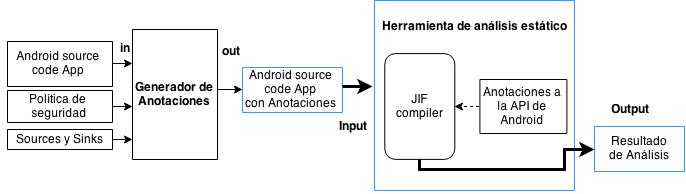
\includegraphics[width=9cm]{desing3Real-2-2-azul.jpg} 
		\end{center}
	\end{figure}
\end{frame}

\subsection{Jif}
\begin{frame}{Características de Jif}
\begin{itemize}
  \item Lenguaje tipado de seguridad.
  \item Extensiones de seguridad al lenguaje java.
  \item Restricciones para uso de la información.
  \item Análisis de flujo de información mediante chequeo de etiquetas.
\end{itemize}
\end{frame}
\begin{frame}[fragile]{Características sobresalientes de Jif}
\begin{columns}[T]
\column{2in}
	\begin{itemize}
	  \item Anotar propiedades de seguridad.
	  \item Verificar las propiedades de seguridad.
	  \item Cubrir todas las posibles ramas de ejecución en el análisis.
	  \item Diseñado para aplicativos Java.
	\end{itemize}
\column{2in}{Flujos: explicitos - implícitos }
\begin{lstlisting}[style=base]
	int x,y;
	x = 1;	
	y = 4 + x;
\end{lstlisting}
\begin{lstlisting}[style=base]
	void foo(a){
	int x;
	if(a > 10)
		x = 1;
	else
		x = 2;
	printf(x);
	}
\end{lstlisting}
\end{columns}

\end{frame}

\subsection{Propuesta - Especificaciones}
\begin{frame}[fragile]{Política de Seguridad}
\begin{columns}[T]
\column{1.5in}
	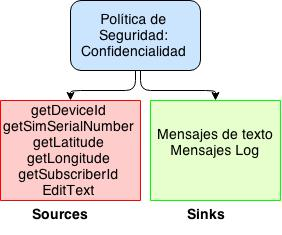
\includegraphics[width=4cm]{Politica.jpg} 
	\pause
\column{2.5in}
\begin{lstlisting}[style=base]
	String imei = @getDeviceId()@;
	<sendTextMessage>(imei);
\end{lstlisting}
\pause
\begin{lstlisting}[style=base][frame=single]
String passwd = @EditText@.getText();
boolean passwdOk = false;
if(passwd.equals("superSecure"))
	passwdOk = true;
if(passwdOk)
	<Log>.i("INFO","Password correcto");
else
	<Log>.i("INFO","Password incorrecto");
\end{lstlisting}
% \begin{lstlisting}[style=base][frame=single]
% String passwd = @EditText@.getText();
% boolean passwdOk = false;
% if(passwd.equals("superSecure"))
% 	passwdOk = true;
% 	
% if(passwdOk)
% 	<Log>.i("INFO","Password correcto");
% else
% 	<Log>.i("INFO","Password incorrecto");
% \end{lstlisting}
\end{columns}
\end{frame}

\begin{frame}[fragile]{Anotaciones Propuestas}
\begin{columns}[T]
\column{1.5in}{DLM de Jif}
\begin{mdframed}
\scriptsize{
\textbf{Principales}\newline
Autoridad
}
\end{mdframed}
\vspace{-0.5em}
\begin{mdframed}
\scriptsize{
\textbf{Políticas}\newline
{dueño: lista-lectores}
}
\end{mdframed}
\vspace{-0.5em}
\begin{mdframed}

\scriptsize{
\textbf{Etiquetas}\newline}
\begin{lstlisting}[style=base2][
int code; 
int {Alice:} code; 
\end{lstlisting}
\end{mdframed}
\pause

\column{2in}
\begin{mdframed}
\scriptsize{
\textbf{Autoridad máxima}\newline
El Principal \emph{\textcolor{red}{Alice}} representa la máxima autoridad del
programa.}
\end{mdframed}
\vspace{-0.5em}

\begin{mdframed}
\scriptsize{
\textbf{Política para anotar información con nivel de seguridad alto:}
\vspace{-0.5em}
\begin{lstlisting}[style=base2]
@{Alice:}@
\end{lstlisting}
\vspace{-0.5em}
Sólo la autoridad máxima del programa podrá leer la información. 
}
\end{mdframed}
\vspace{-0.5em}

\begin{mdframed}
\scriptsize{
\textbf{Política para anotar información con nivel de seguridad bajo:}
\vspace{-0.5em}
\begin{lstlisting}[style=base2]
<{ }>
\end{lstlisting}
\vspace{-0.5em}
No se define un Principal la información podrá leerse por todos. }
\end{mdframed}
\end{columns}
\end{frame}

\begin{frame}{Anotaciones a la API} 
\begin{block}{Flujo de información en la API}
	\begin{itemize}
	  \item La API posibilita el acceso de la app a sources y Sinks.
	  \item Se generan flujos de información.
	  \item Controlar flujos de información entre sources y sinks.
	\end{itemize}
\end{block}
\pause
\begin{block}{Sources y sinks definidos en la API}
	\begin{itemize}
	  \item getDeviceId (método source) $\rightarrow$ TelephonyManager
	  \item Mensajes de texto (sinks) $\rightarrow$ SmsManager
	\end{itemize}
\end{block}
\end{frame}

\begin{frame}[fragile]{Anotaciones a la API}
\begin{block}{Flujo explícito}
\begin{center}
\begin{lstlisting}[style=base2]
String @{Alice:}@imei = getDeviceId();
String <{}> pub = imei;
\end{lstlisting}
\end{center}
\end{block}
\pause
\begin{block}{Flujo implícito}
\begin{center}
\begin{lstlisting}[style=base2][frame=single]
String @{Alice:}@passwd = EditText.getText();
boolean <{}>passwdOk = false;
if(passwd.equals("superSecure"))
	passwdOk = true;
	
if(passwdOk)
	<Log>.i("INFO","Password correcto");
else
	<Log>.i("INFO","Password incorrecto");
\end{lstlisting}
\end{center}
\end{block}
\end{frame}
